\chapter{The Condition (Sophie)}
\label{ch:medicalInfo}
Obstructive Sleep Apnoea (OSA) - sometimes called hypersomnia sleep apnoea syndrome, occlusive sleep apnoea ~\cite{whitelaw1993characteristics}, sleep disordered breathing ~\cite{sleepdisorderedbreathing}, hyperventilation syndrome or Pickwickian Syndrome (although the latter three terms are discouraged because they are also used to describe other disorders)  - is a sleep disorder characterised by repetitive blockages in the upper airway during sleep, but with inspirational effort. These blockages can be apnoeas - full closure - or hypopnoeas  - partial closure. Both cause a restriction in airflow, which can lead to reduction in oxygen saturation and frequent arousal in order to re-establish airflow ~\cite{american2001international}.

The upper airways include the nasal cavity, oral cavity, and pharynx - the area behind the tongue (see Figure \ref{fig:Sagittal-Face}). Blockages mainly occur in the pharynx which is usually held open by the pharyngeal dilator muscles. Although these relax during sleep, in a healthy subject they are still able to maintain airflow, however in an OSA sufferer they provide insufficient force to prevent collapse ~\cite{fogel2004sleep}. Collapse only occurs during inspiration and is due to negative pharyngeal pressure. During rapid eye movement (REM) sleep there is further relaxation of the pharyngeal dilator muscle which can lead to longer apnoea and hypopnoea events. 

\begin{figure}[h]
\centering
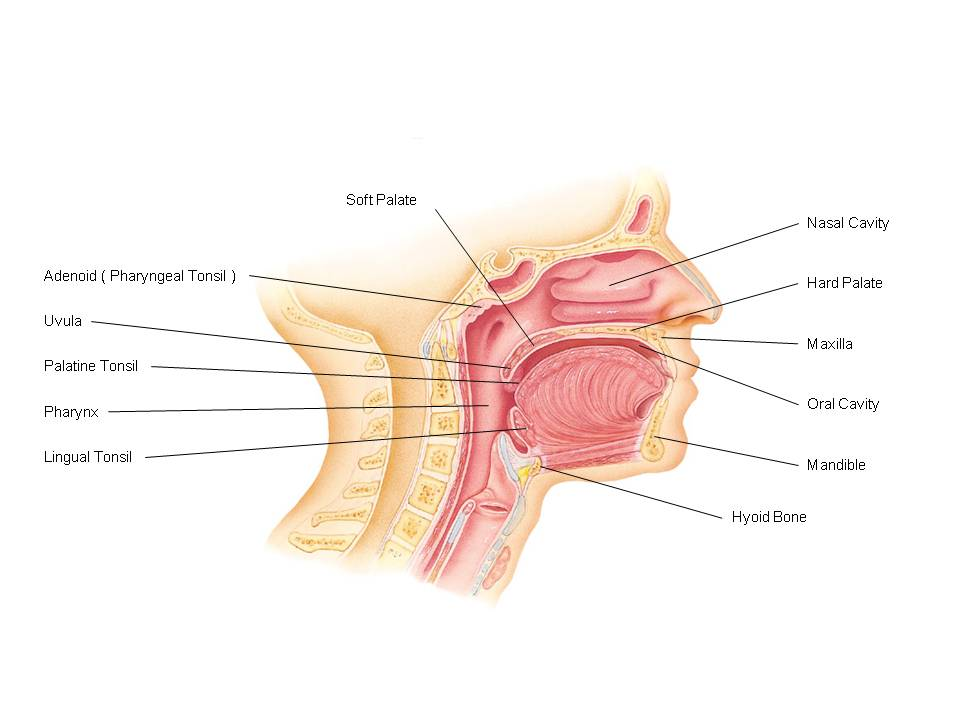
\includegraphics[width=0.8\textwidth]{drawings/Sagittal-Face}
\caption{Sagittal View of the Face to show Upper Airways ~\cite{sagittalface}}
\label{fig:Sagittal-Face}
\end{figure}
Many factors affect the likelihood a patient suffers with OSA, however one thing is consistent in almost all cases; the pharyngeal upper airway size is smaller than in normal patients and often more elliptical, with the long axis directed anterior-posterior rather than laterally as it is in non sufferers, which alters the pharyngeal dilator muscle orientation leading to a mechanical disadvantage. This can have a number of causes including fat deposits and facial bone structure ~\cite{leiter1996upper}. 
Overweight and obese patients often have fat deposits lateral to the pharynx, not always substantial, but their positioning creates or reinforces elliptical shape, pharyngeal orientation and reduction in size. 

The main element of facial bone structure that influence upper airway size is the positioning and size of the maxilla and mandible (upper and lower jaw bones), these can influence the airway size in two ways: micrognathia where the jaws are undersized, and retrognathia (or overbite) where the mandible is set back compared to the maxilla. In both of these cases the tongue sits further back in the mouth, increasing the tendency to block airflow. Lower positioning of the hyoid bone and Brachycephaly, where the head is wider than it is tall, can have a similar effect ~\cite{lowe1995cephalometric}.

Abnormal facial tissues can also have an effect; large tonsils and adenoids, elongated or enlarged uvula (the dangly bit at the back of the mouth, see Figure \ref{fig:Anterior-View-Mouth}), macroglossia (enlarged tongue), high arched or narrow hard palate, and reduced nasal patency (cross sectional area), possibly caused by nasal abnormalities, all have been shown to factor ~\cite{schwab1995upper}.

\begin{figure}[h]
\centering
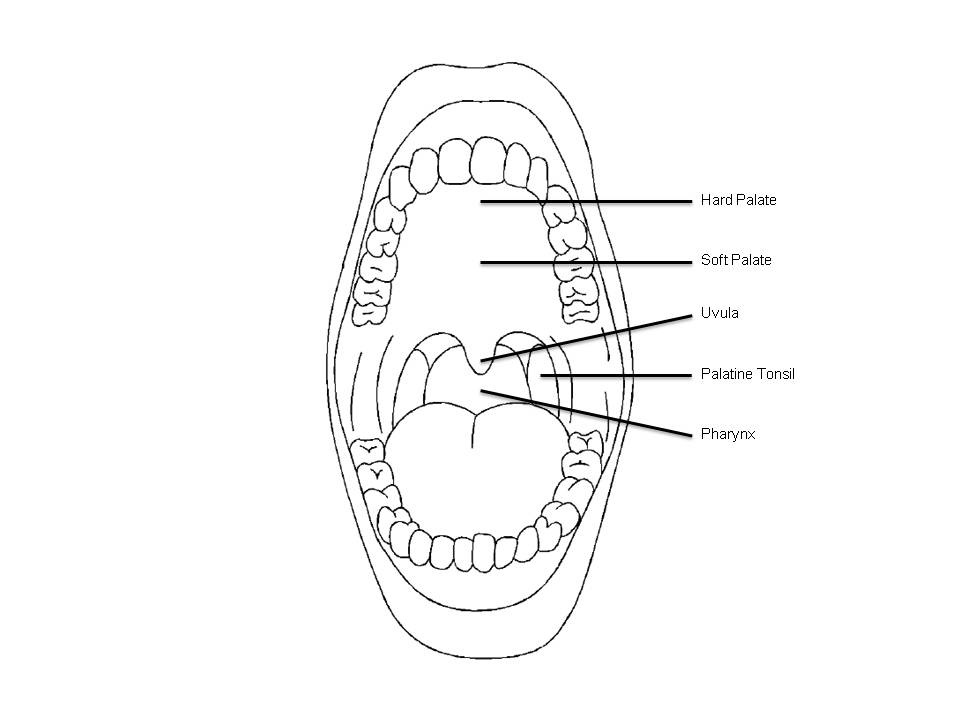
\includegraphics[width=0.5\textwidth]{drawings/Anterior-View-Mouth}
\caption{Anterior View of the Mouth to show Upper Airway Tissues~\cite{anteriormouth}}
\label{fig:Anterior-View-Mouth}
\end{figure}

Other factors include lying supine (on one’s back) where gravity causes the tongue to fall into the airway. Some drugs including alcohol relax the pharyngeal dilator muscles more than just the effects of sleep, worsening OSA. Smoke irritates tissues including those in the upper airways, swelling them causing a narrowing of the airway ~\cite{apneosotherfactors}.

 Severity of the Condition can be measured in two ways: AHI and RDI. AHI or Apnoea Hypopnoea Index counts the average number of apnoeas and hypopnoeas per hour asleep. The severity is then classified as minimal if AHI \textless\ 5, mild if 5 $\leq$ AHI \textless\ 15, moderate 15 $\leq$ AHI \textless\ 30 and severe AHI $\geq$ 30. RDI or Respiratory Disturbance Index is similar but also includes respiratory-effort related arousals (RERAs) in the count ~\cite{AHI}. The same classifications are used for RDI as for AHI; however this can be unhelpful given that the RDI is likely to be higher than AHI for the same patient ~\cite{epstein2009clinical}.

